\chapter{試作2号機:インスタンス認識ハンドの開発}
\newpage

\section{要求仕様}
1号機の課題の中で特に,把持機構の自由度が小さい事と,物体の正確な識別が不可能である問題は実用化の障害となる.
そこで2号機ではこれら2点の課題を克服したロボットハンドを開発する.

ハードウェアとして,1号機では対象に近づきグリップすることをゴールとしたが,実使用を考えると物を持ち帰って次の動作をすることが要求される.そこで2号機では手首機構を重視して,より多彩な動きを実現するためアクチュエータを増やし,把持機構の自由度を上げる必要がある.グリッパとして,指定した点で掴む,またグリッパの中心軸で左右対称に掴む,という動作を可能にする機構が必要である.また,掴む時の把持点決定及び指定した点を掴めるようアクチュエータで調整できることが要求される.そして掴んだ後の物体の滑り防止機構が必要である.
物体をピックアップするために,環境把握に加えて物体との距離を正確に捉える必要がある.

ソフトウェアとして,1号機に搭載したスマートフォンでは環境認識に1秒を要したため,より高速に演算できる計算リソースが要求される.多自由度化に伴いより多くのアクチュエータを制御するため,スマートフォンではなくGPUを搭載したデバイスで学習・推論を行う必要がある.また,1号機では色のみの認識であったが,把持対象物を"物体"として認識し,複数種類に拡張して識別できることが要求される.


\section{機構設計・機体デザイン}
環境把握と対象物との距離を測るためにRGBカメラとデプスカメラを両方搭載したIntel社のRealSenseを用いた.
対象物を持ち上げるために腕に関節を1つ加え,地面から垂直に対象物を挙上できるようにした.
把持中心点を正確に掴むため,2指対立タイプの一般的な形状のグリッパとした.
把持中心位置の制御では,高精度化のためにラック\&ピニオンを用いてサーボモータの回転を水平運動に変換にし,腕を進行方向と垂直な方向にスライドできるようにした.

以上を考慮して\fig{2号機CAD}に示すようなフレームを3DCAD(123D Design Autodesk社を使用)で設計した.また,ロボットハンドの向きは\fig{2号機CAD}に示す,ソフトウェアでの画像(配列)の向きと同様の定義とする.

\begin{figure}
    \centering
    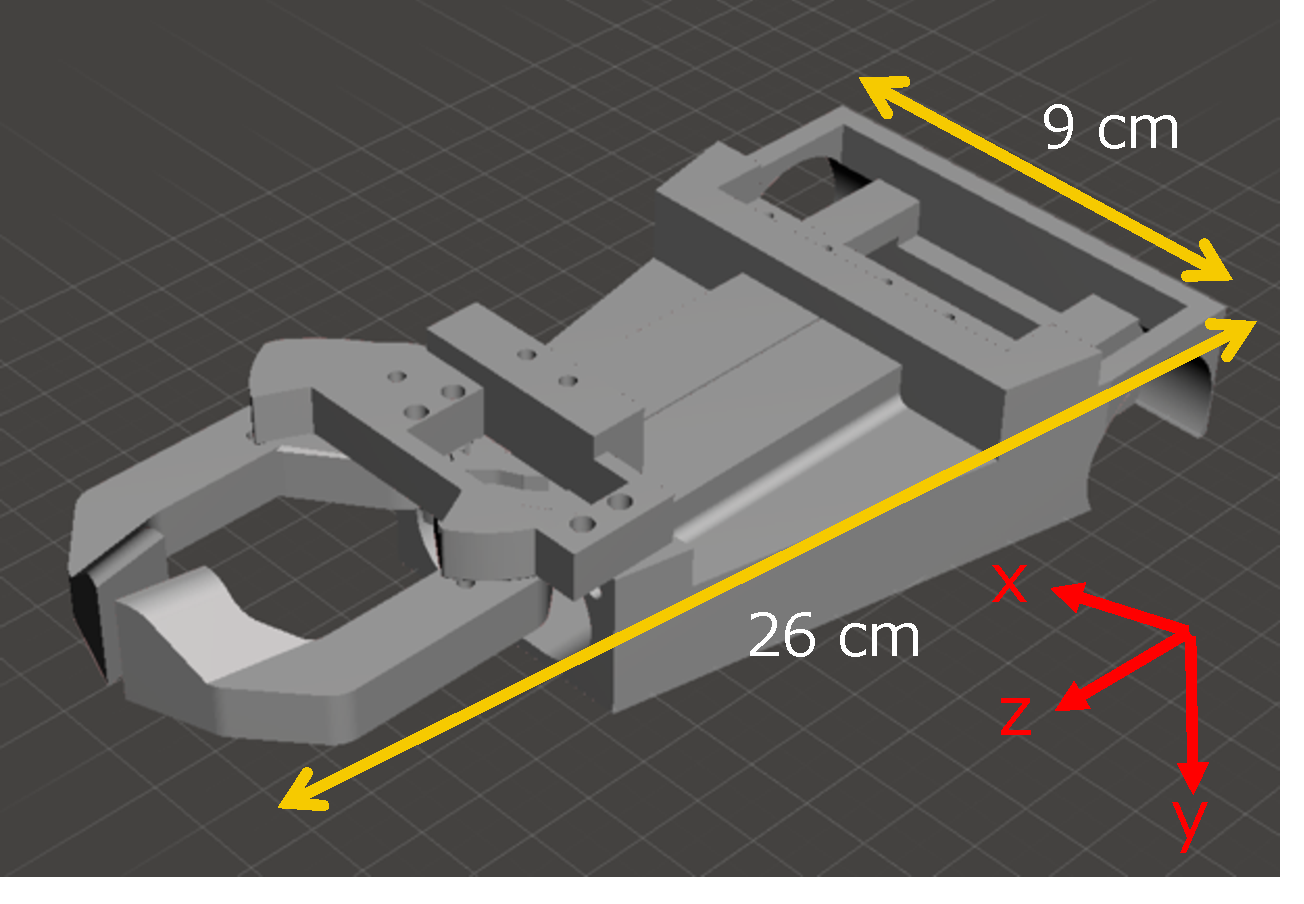
\includegraphics[width=\linewidth]{figure/chapter4/2号機CAD}
    \caption{3DCAD image of prototype No.2}
    \label{fig:2号機CAD}
\end{figure}


\section{制御アルゴリズム}
2号機では強化学習ではなく比例制御の考え方を利用した手法及びルールベースによって対象物のピックアップを行った.

\begin{figure}
    \centering
    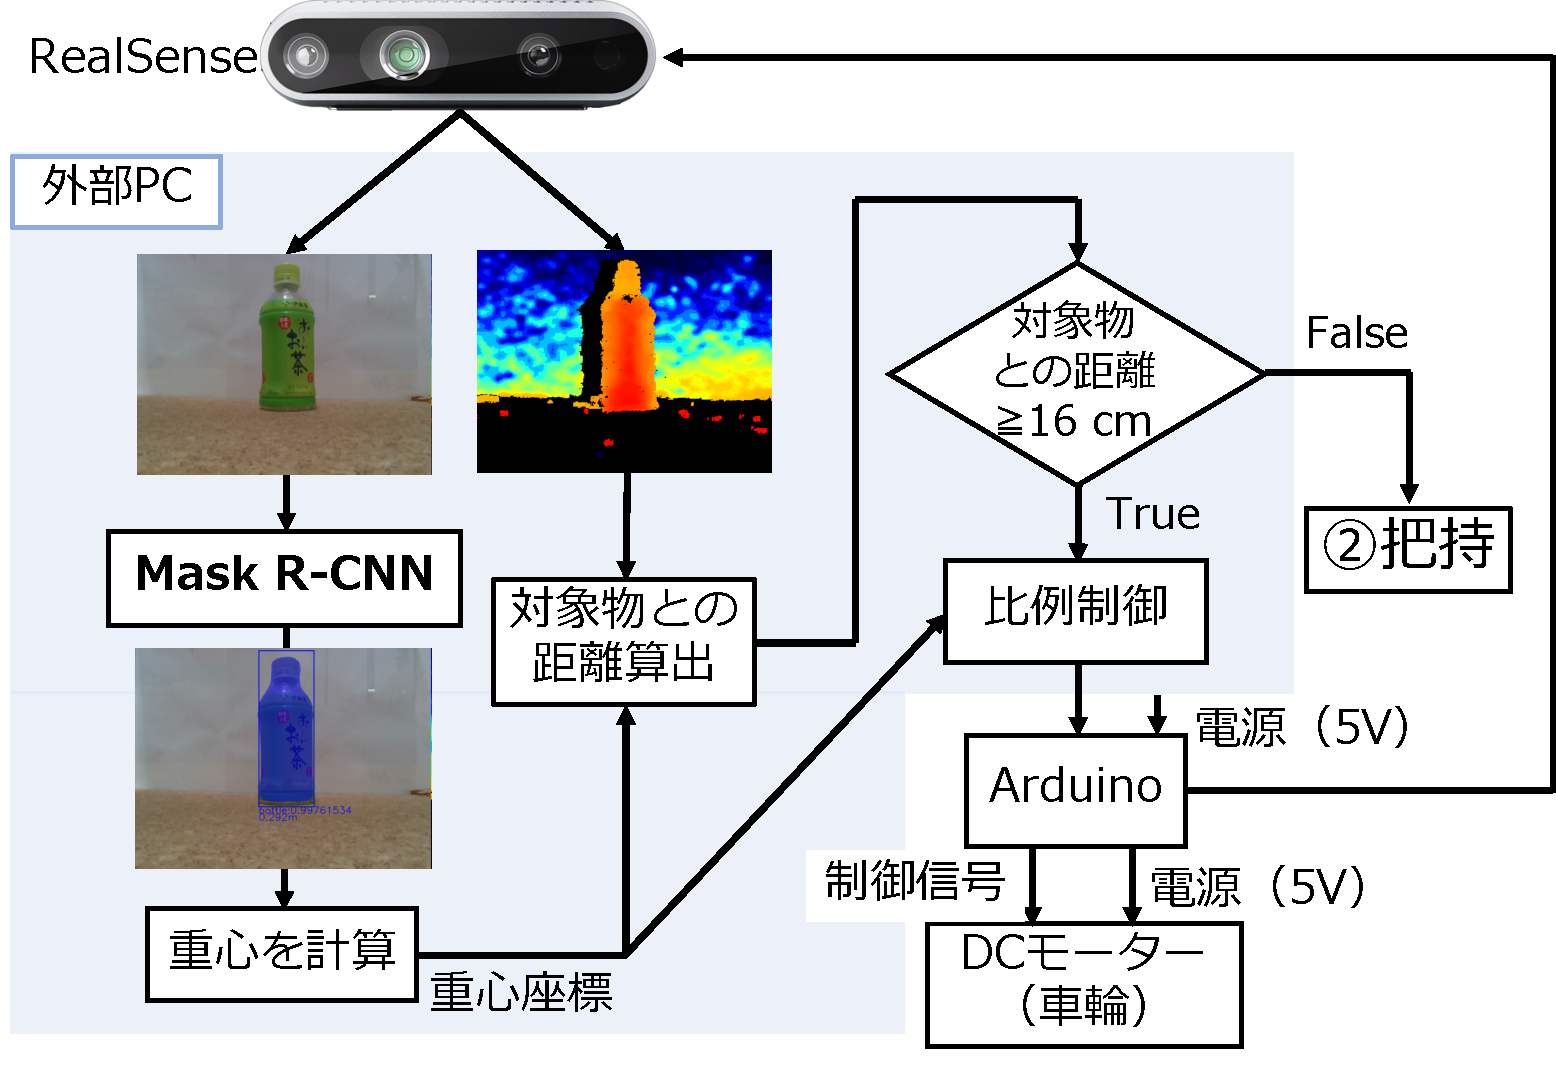
\includegraphics[width=0.7\linewidth]{figure/chapter4/2号機制御図_接近}
    \caption{Block diagram of tracking objects task.}
    \label{fig:2号機接近}
\end{figure}


接近動作では2段階に分けて行った.まず対象物までのラフな接近について述べる(\fig{2号機接近}).
インスタンスセグメンテーションにより物体を検出し,対象物のマスクを取得し重心を計算した.その重心がロボットハンドの中心軸に来るように,左右輪のスピードをそれぞれ独立に以下の更新式によって制御しながら接近させた.
\begin{lstlisting}[caption=接近アルゴリズム, label=code:motor]
r_motor = (1 - error_distance) / 2 * MAX_SPEED
l_motor = (1 + error_distance) / 2 * MAX_SPEED
\end{lstlisting}
ここで\texttt{MAX\_SPEED}はモーターの最大スピードで今回は100とした.\texttt{error\_distance}はロボットハンドと対象物との画像内におけるx軸方向のズレを画像の横の長さの半分で規格した値であり,-1から1の値をとる.そして対象物からRealSenseのデプス測定限界である20 cm程度まで近づいたら停止させた.

\begin{figure}
    \centering
    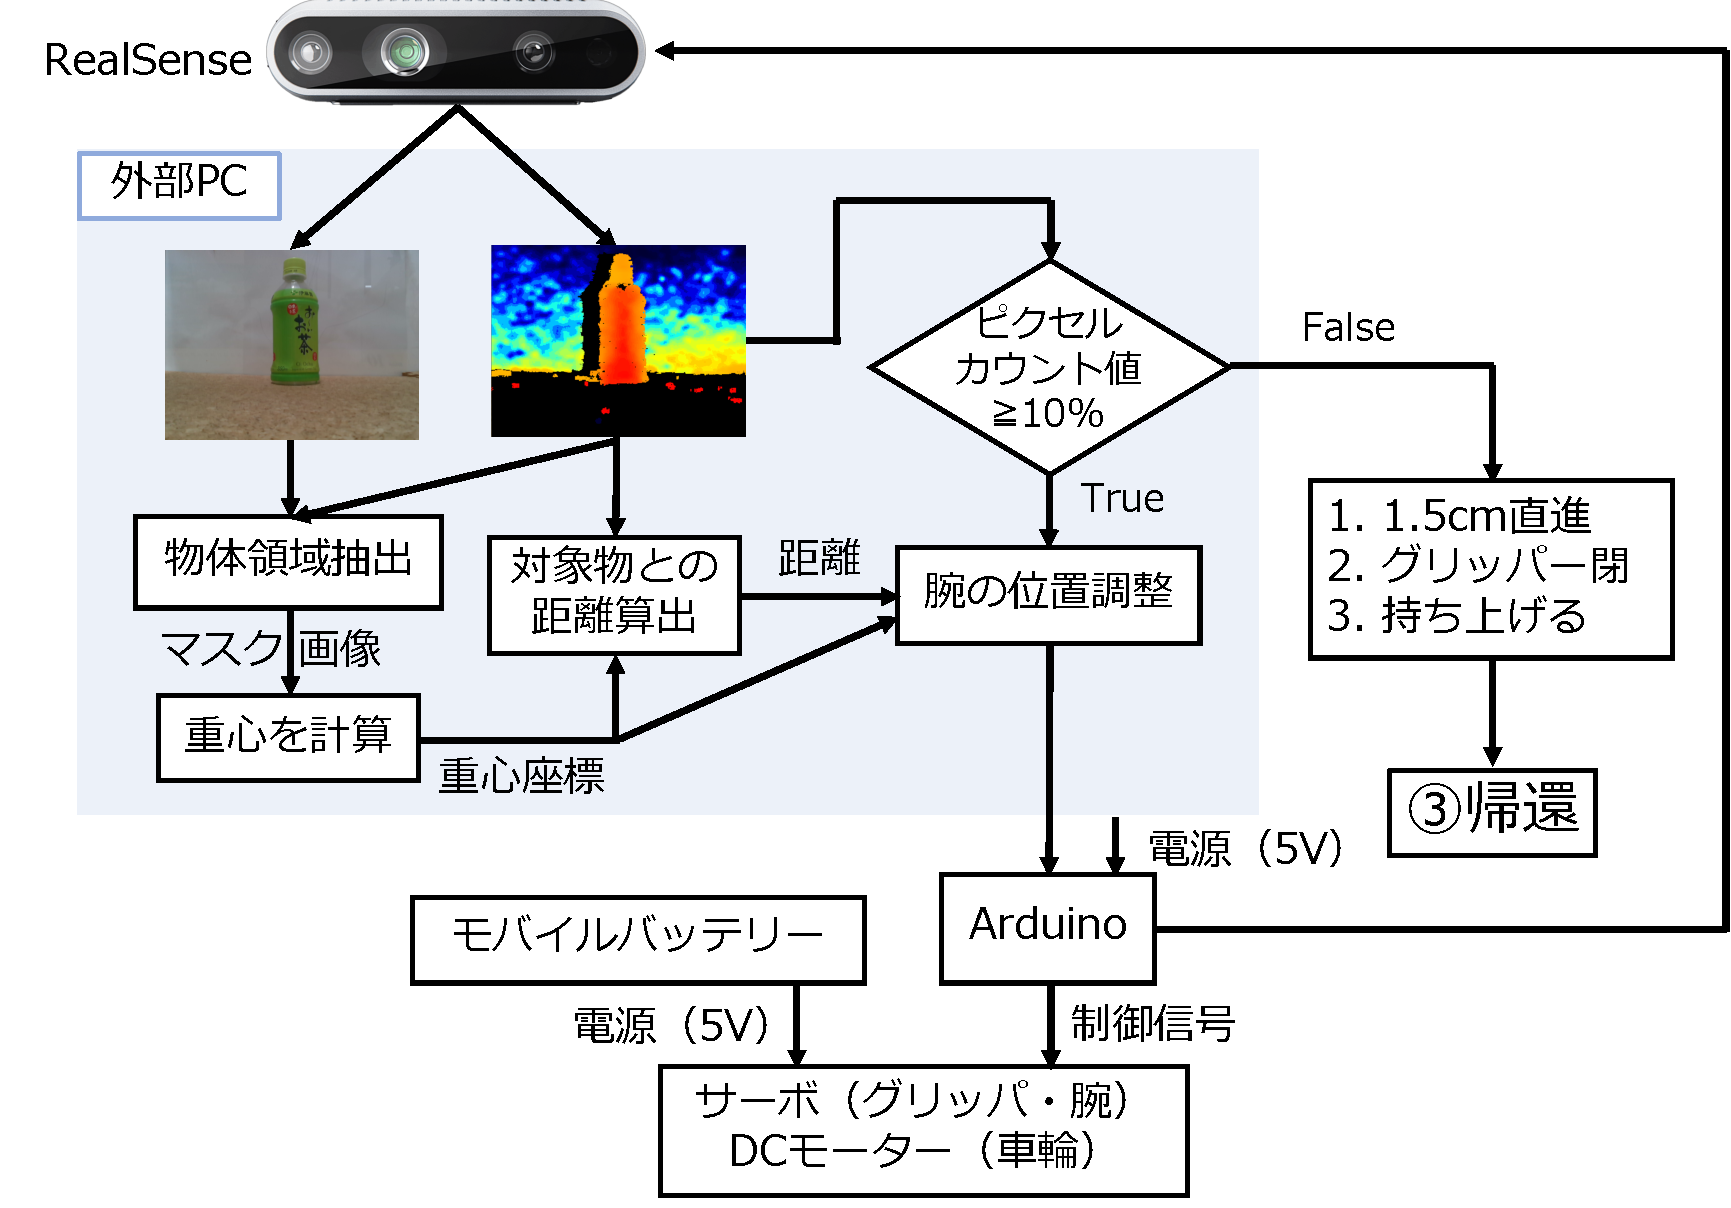
\includegraphics[width=0.7\linewidth]{figure/chapter4/2号機制御図_把持}
    \caption{Block diagram of grasping objects task.}
    \label{fig:2号機把持}
\end{figure}

次に対象物への把持動作に向けた微調整および把持動作について述べる(\fig{2号機把持}).
対象物の重心にハンドの把持中心が来るように横方向にラックピニオンで修正を加えた.この時,画像におけるピクセル間距離を実距離に変換し,重心とハンド中心の変位をなるべく小さくするようにサーボを動かした.そしてデプスカメラが対象物に覆われて見えなくなるまで(デプス画像の現フレームとのピクセル数比を取り,10\%以下になるまで)直進させた.
そこからさらにグリッパのより内側に対象物を収めるため4 cm直進させ,グリッパを閉じさせた.その後腕を上げ物体を持ち上げ,この際のデプス画像を保持しておいた.そこから1秒ごとにデプス画像の現フレームとのピクセル数比を取り,50\%以下であったら失敗とし,5秒落とさず維持したら把持成功とした.

\begin{figure}
    \centering
    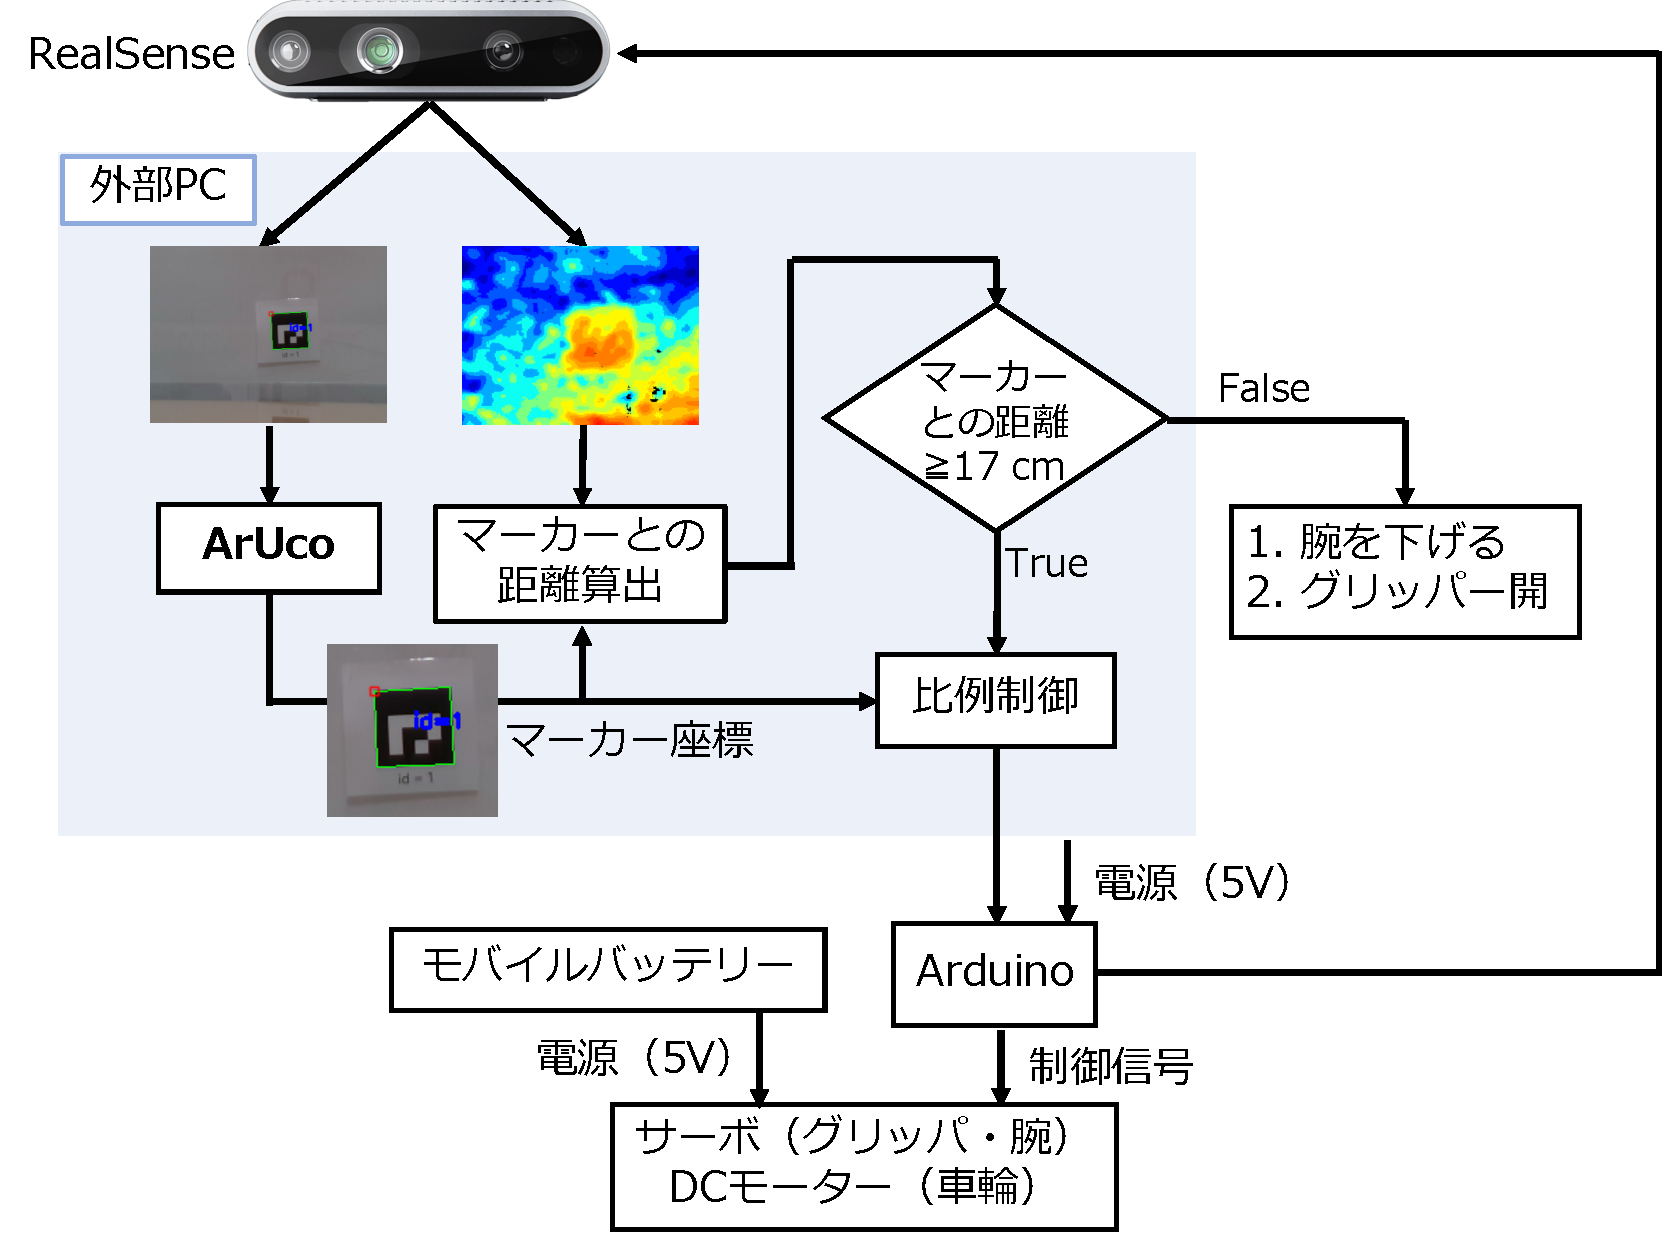
\includegraphics[width=0.7\linewidth]{figure/chapter4/2号機制御図_AR}
    \caption{Block diagram of get back home position task.}
    \label{fig:2号機AR}
\end{figure}

最後に,把持をした物体を運搬する動作について述べる(\fig{2号機AR}).
把持が成功したらコード\ref{code:motor}と同様の制御でホームポジションまで戻った.ホームポジションの認識にはARマーカーを使用した.

なお,Arduinoとのシリアル通信では1回に2byteまでしか送信できず,String型でモーター5台の情報を送信すると遅延や読み飛ばしが発生した.そこで2号機ではモーターの取る値をデジタル化し情報を圧縮してByte型で送信するようにした.実際に取る値と送信bit信号の対応表を\tab{2号機信号表}に示す.

\begin{table}
    \centering
    \caption{Convert value of motor speed or servo degree to bit signal.}
    \begin{tabular}{cccc}\toprule
        Actuator & Bit signal & Value @ Arduino & Value @ Python \\ \midrule
        Forward right DC motor & 000 & 0--100(step 5) & 0--20  \\ 
        Forward left DC motor & 001 & 0--100(step 5) & 0--20 \\ 
        Grip servo & 010 & 0 / 100 & 0 / 1\\ 
        Vertical swing servo & 011 & 0 / 100 & 0 / 1\\ 
        Horizontal slide servo & 100 & 0--180 (step 10) & 0--18 \\ 
        Terminate & 101 & 0 / 1 & 0/1 \\ 
        Backward right DC motor & 110 & 0--100(step 5) & 0--20 \\ 
        Backward left DC motor & 111 & 0--100(step 5) & 0--20 \\ \bottomrule
    \end{tabular} 
    \label{tab:2号機信号表}
\end{table}

Bit signalが駆動させるアクチュエータを2進数で示しており,動かす値をValue @ Pythonに示す10進数を5桁の2進数に変換してそれぞれをドッキングして8桁の2進数として1byteのデータをシリアル送信した.

RealSenseおよびArduinoの制御はG-DEP社のDeepLearning BoxII(Ubuntu16.04)を使用し,計算リソースはNVIDIA社のGPU(TITAN RTX)を使用した.
プログラムは筆者のGitHub\footnote{\url{https://github.com/yumion/onodera-lab/tree/master/robotHandV2}}で公開している.


\subsection{RealSenseを使用したカメラ画像内における実距離推定}
把持位置を制御する際,画像内のピクセル座標ではなく実世界におけるx軸方向やy軸方向の長さを知る必要がある(z軸方向はデプスカメラで測距可能).そこで,ピクセル間距離から実距離を回帰処理によって求めた.また,カメラから測る対象物までの距離にも依存するため,RealSenseを用いて距離依存性についても回帰処理を行い,2段階で求めた.

具体的には,壁に30cm定規を置きカメラは壁と平行になるよう設置した.壁からカメラの距離$z$(cm)を変えながら定規の目盛りのピクセル座標を取得し,横軸にピクセル差分$\Delta \rm{pixel}$,縦軸にそのピクセルに対応する定規の目盛り幅$\Delta x$(cm)をプロットした(\fig{pix2dist}).また,各$z$で線形回帰を行ったあと横軸に壁からカメラの距離$z$,縦軸に傾き$a$をプロットし線形回帰を行い,全ての距離$z$におけるピクセル間距離を求めた(\fig{depth2grad}).

\begin{figure}
    \centering
    \begin{minipage}{0.49\hsize}
        \centering
        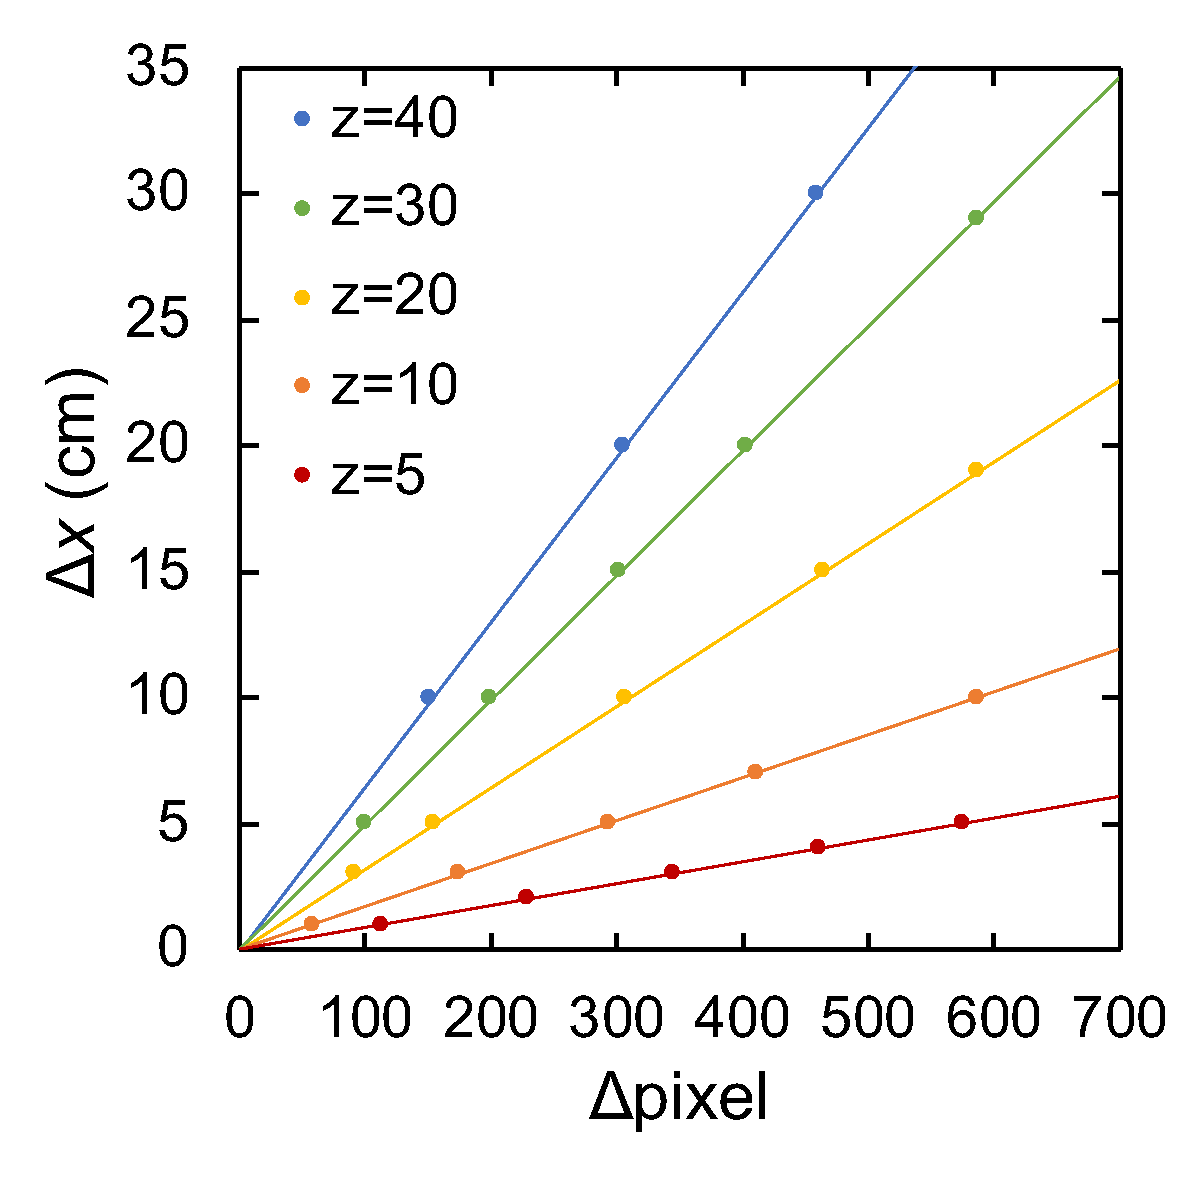
\includegraphics[width=\linewidth]{figure/chapter4/pixel2distance}
        \subcaption{Pixel to Distance}
        \label{fig:pix2dist}
    \end{minipage}
    \begin{minipage}{0.49\hsize}
        \centering
        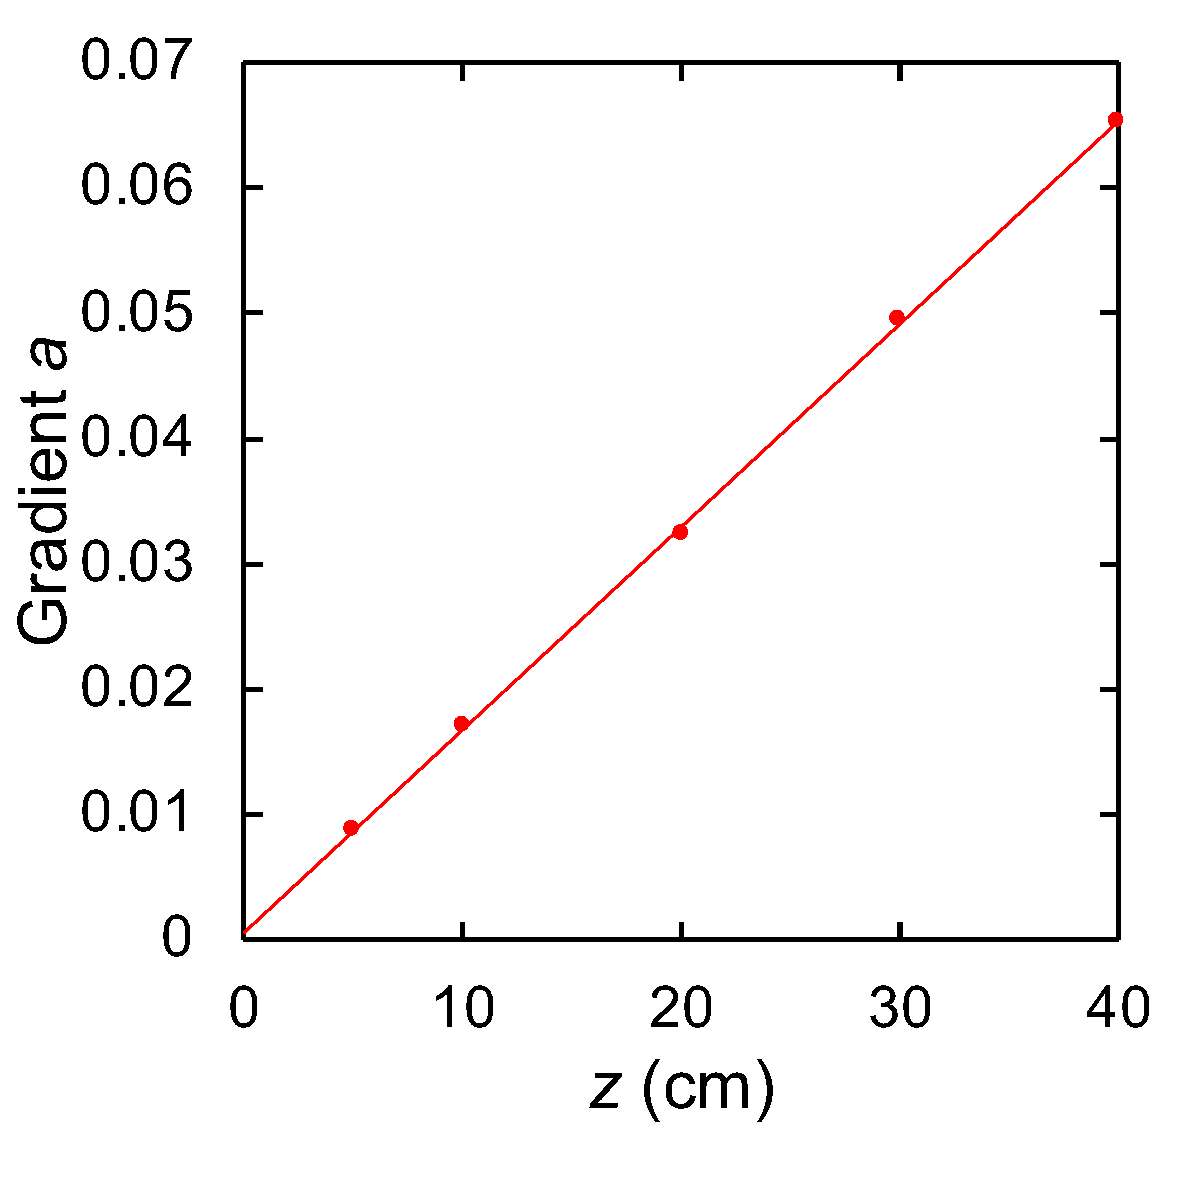
\includegraphics[width=\linewidth]{figure/chapter4/depth2gradient}
        \subcaption{Dependency of depth}
        \label{fig:depth2grad}
    \end{minipage}
    \caption{Convert pixel-wise to distance in real.}
    \label{fig:pix2distance}
\end{figure}

\begin{figure}
    \centering
    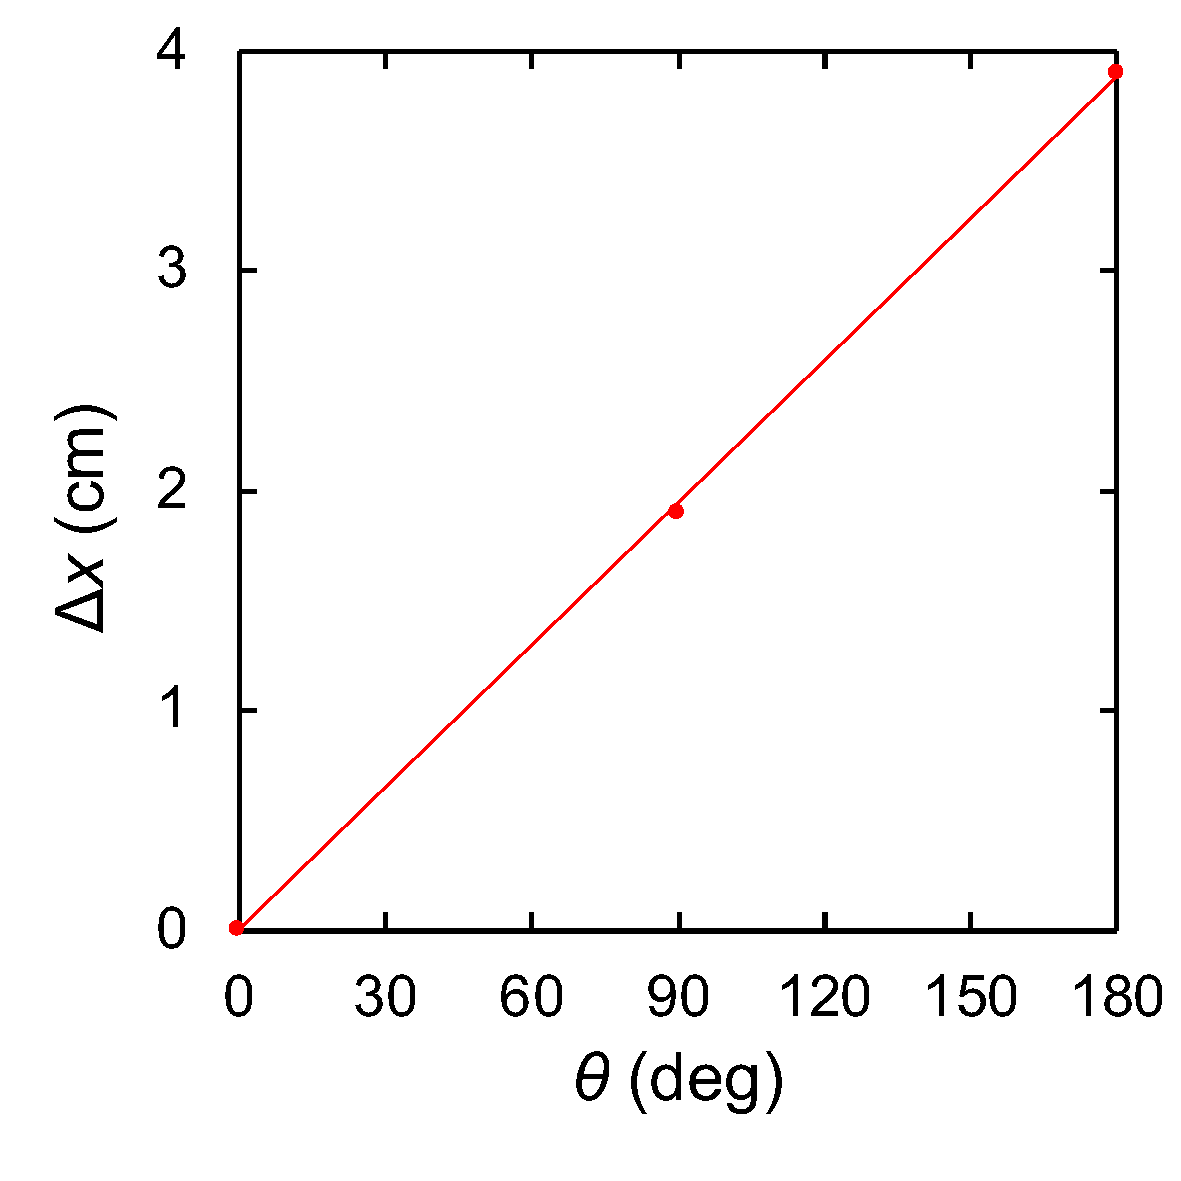
\includegraphics[width=0.5\linewidth]{figure/chapter4/servo2distance}
    \caption{Convert servo input to distance.}
    \label{fig:servo2dist}
\end{figure}

以上から,実距離$\Delta x$はピクセル間距離$\Delta \rm{pixel}$とカメラと対象物の距離$z$を用いて
\begin{align}\label{eq:ピクセル間距離}
\Delta x \simeq (0.0016z + 0.0006) \cdot \Delta \rm{pixel}
\end{align}
と推定できる.

また,ラック\&ピニオンの回転から水平移動に変換するためには,サーボが0\deg -- 180\deg まで可動するため,その移動最大距離を測定しておき(4cm),各角度における0\deg からの移動量をプロットし線形回帰する(\fig{servo2dist})ことで以下のように求められる.

\begin{align}\label{eq:スライド角度}
\Delta x \simeq 0.0216 \theta
\end{align}
ここで,$\Delta x$は水平移動距離(cm),$\theta$はサーボの回転角度(deg)である.
\eq{ピクセル間距離}と\eq{スライド角度}から
\begin{align}
\theta & \simeq \dfrac{\Delta x}{0.0216} \\
& = \dfrac{0.0016z + 0.0006}{0.0216} \Delta \rm{pixel} \\
\end{align}
として画像からサーボを何度動かせば良いかが分かる.なお,実装上はサーボの可動範囲が0\deg -- 180\deg を考慮して
\begin{lstlisting}[label=code:servo]
vertical_deg =\
(max(min(vertical_pos // 0.0216, 90), -90) + 90) // 10
\end{lstlisting}
とすることで入力の最小0,最大を180とし,サーボへの入力が0の時に真ん中である90\deg とし,それを1/10にデジタル化して送信する.\texttt{vertical\_pos}は$\Delta x$(cm),\texttt{vertical\_deg}は$\theta$(deg)である.


\subsection{Mask R-CNNを用いた物体のセグメンテーションと測距}\label{sec:mrcnn学習}
2号機では,物体の識別のためにインスタンスセグメンテーションの手法の1つであるMask R-CNNを用いた.COCO2014およびCOCO2017のデータセット\footnote{\url{http://cocodataset.org}}で学習した.
学習した結果を\tab{MSCOCO評価}に示す.

\begin{table}[H]
    \centering
    \caption{Results of Mask R-CNN validated by COCO.}
    \begin{tabular}{ccccc}\toprule
        & \multicolumn{2}{c}{Object Detection} & \multicolumn{2}{c}{Segmentation} \\ 
        & 2014 & 2017 & 2014 & 2017 \\ \midrule
        $\rm{AP}^{\rm{IoU}=0.50:0.95} \u{maxDets=100} @Area=all$ & 0.352 & 0.227 & 0.334 & 0.243 \\ 
        $\rm{AR}^{\rm{IoU}=0.50:0.95} \u{maxDets=100} @Area=all$ & 0.438 & 0.299 & 0.405 & 0.301 \\ 
        FPS & 4.078 & 3.880 & 4.013 & 4.002 \\ \bottomrule
    \end{tabular} 
    \label{tab:MSCOCO評価}
\end{table}

また,デプスカメラを用いて検出した物体の距離も同時に測定した.Mask R-CNNの出力であるマスクの重心を求め,その座標までの距離をデプスカメラで測定した.\fig{maskrcnn例}にCOCO2014で学習済みモデルを使用した物体検出およびその物体までの測距の例を示す.

\begin{figure}[H]
    \centering
    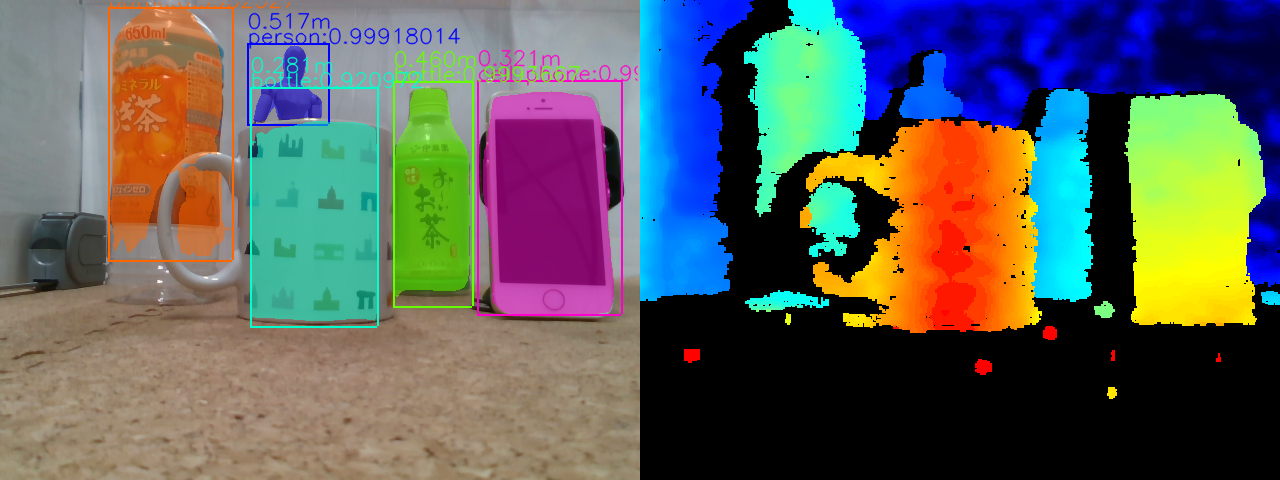
\includegraphics[width=0.7\linewidth]{figure/chapter4/MaskR-CNN_screenshot}
    \caption{Examples of Mask R-CNN inference.}
    \label{fig:maskrcnn例}
\end{figure}

このように,物体のセグメンテーションが完璧ではなくても対象物の重心はおおよそ把握できるため,IoUよりもPrecisionを重視し物体検出におけるfpsが高いCOCO2014の学習モデルを使用した.


\section{実機作製}

\tab{2号機部品}に2号機作製に当たって使用した部品をまとめた.

\begin{table}[H]
    \centering
    \caption{Components of prototype No.2}
    \begin{tabular}{cc}\toprule
        本体フレーム & PLA(赤) \\
        デプスカメラ & RealSense D435i \\ 
        マイコン & Arduino Nano \\ 
        DCモータ & \href{http://akizukidenshi.com/catalog/g/gM-12379/}{STLギヤモータ 栄42D長軸型} \\ 
        サーボモータ & \href{https://hitecrcd.co.jp/products/servo32225/}{HS-225MG} x1,\href{https://hitecrcd.com/products/servos/discontinued-servos-servo-accessories/hsr-5990tg-hmi-ultra-premium-robot-servo/product}{HSR-5990TG} x1,\href{https://hitecrcd.co.jp/products/servo31422s/}{HS-422} x1 \\ 
        バッテリー & モバイルバッテリー \\ 
        タイヤ & \href{https://tamiya.com/japan/products/70194/index.html}{TAMIYA製スパイクタイヤ} \\
        リニアガイド &  \\
        ラック\&ピニオン &  \\ \bottomrule
    \end{tabular} 
    \label{tab:2号機部品}
\end{table}

1号機と同様にロボットハンドのフレームは簡便さと軽さを考慮して3Dプリンタ(Adventure3)で造形した.
\fig{2号機外観}に作製したロボットハンドの外観を示す.サーボモータを3つ使い,それぞれグリッパの開閉,腕のy軸方向への振り上げの関節,腕のx軸方向へのスライドに使用した.グリッパの先端にはゴムをつけてグリップ力を上げた.腕のスライドにはリニアガイドを用いてスムーズに腕が動くようにした.
アクチュエータのバッテリーにはモバイルバッテリーを使用し,フレーム内部に組み込んだ.RealSenseはロボットハンドの土台の先端にネジ止めをした.
RealSenseおよび各アクチュエータの制御は外部のデスクトップPCとArduino Nanoを使用し,有線で接続した.
2号機の総重量は572.27gであった.

\begin{figure}[H]
    \centering
    \includegraphics[width=\linewidth]{figure/chapter4/2号機外観}
    \caption{Appearance of Prototype No.2. Weight is 572.27 g.}
    \label{fig:2号機外観}
\end{figure}


\section{評価方法}
2号機の改良点は対象物の識別性能とより正確な把持動作である.したがってこの2点に関して評価を行った.

COCOデータセットの中で,机の上にあるものを識別・把持できるかを検証した.
今回,対象とした物体は\fig{対象物}に示す5つの物体(4種類)である.また,\tab{対象物}に各対象物の詳細を示す.ロボットハンドの機構上,地面から高さが低い物体は把持ができないため,各対象物は正立させた状態で配置した."cell phone"は背面にクリップを付けて直立させた.
\begin{figure}[H]
    \centering
    
    \begin{minipage}{0.19\columnwidth}
        \centering
        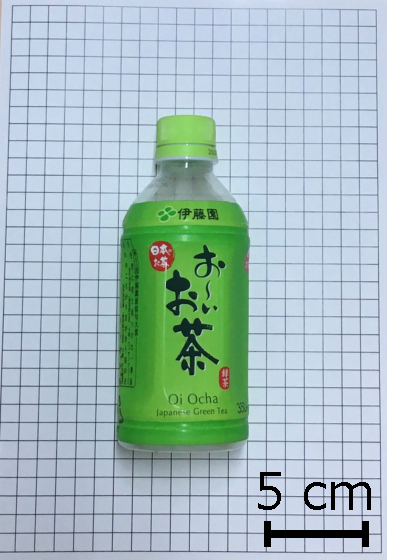
\includegraphics[clip, width=\linewidth]{figure/chapter4/bottle_350ml}
        \subcaption{bottle(350ml)}
    \end{minipage}
    \begin{minipage}{0.19\columnwidth}
        \centering
        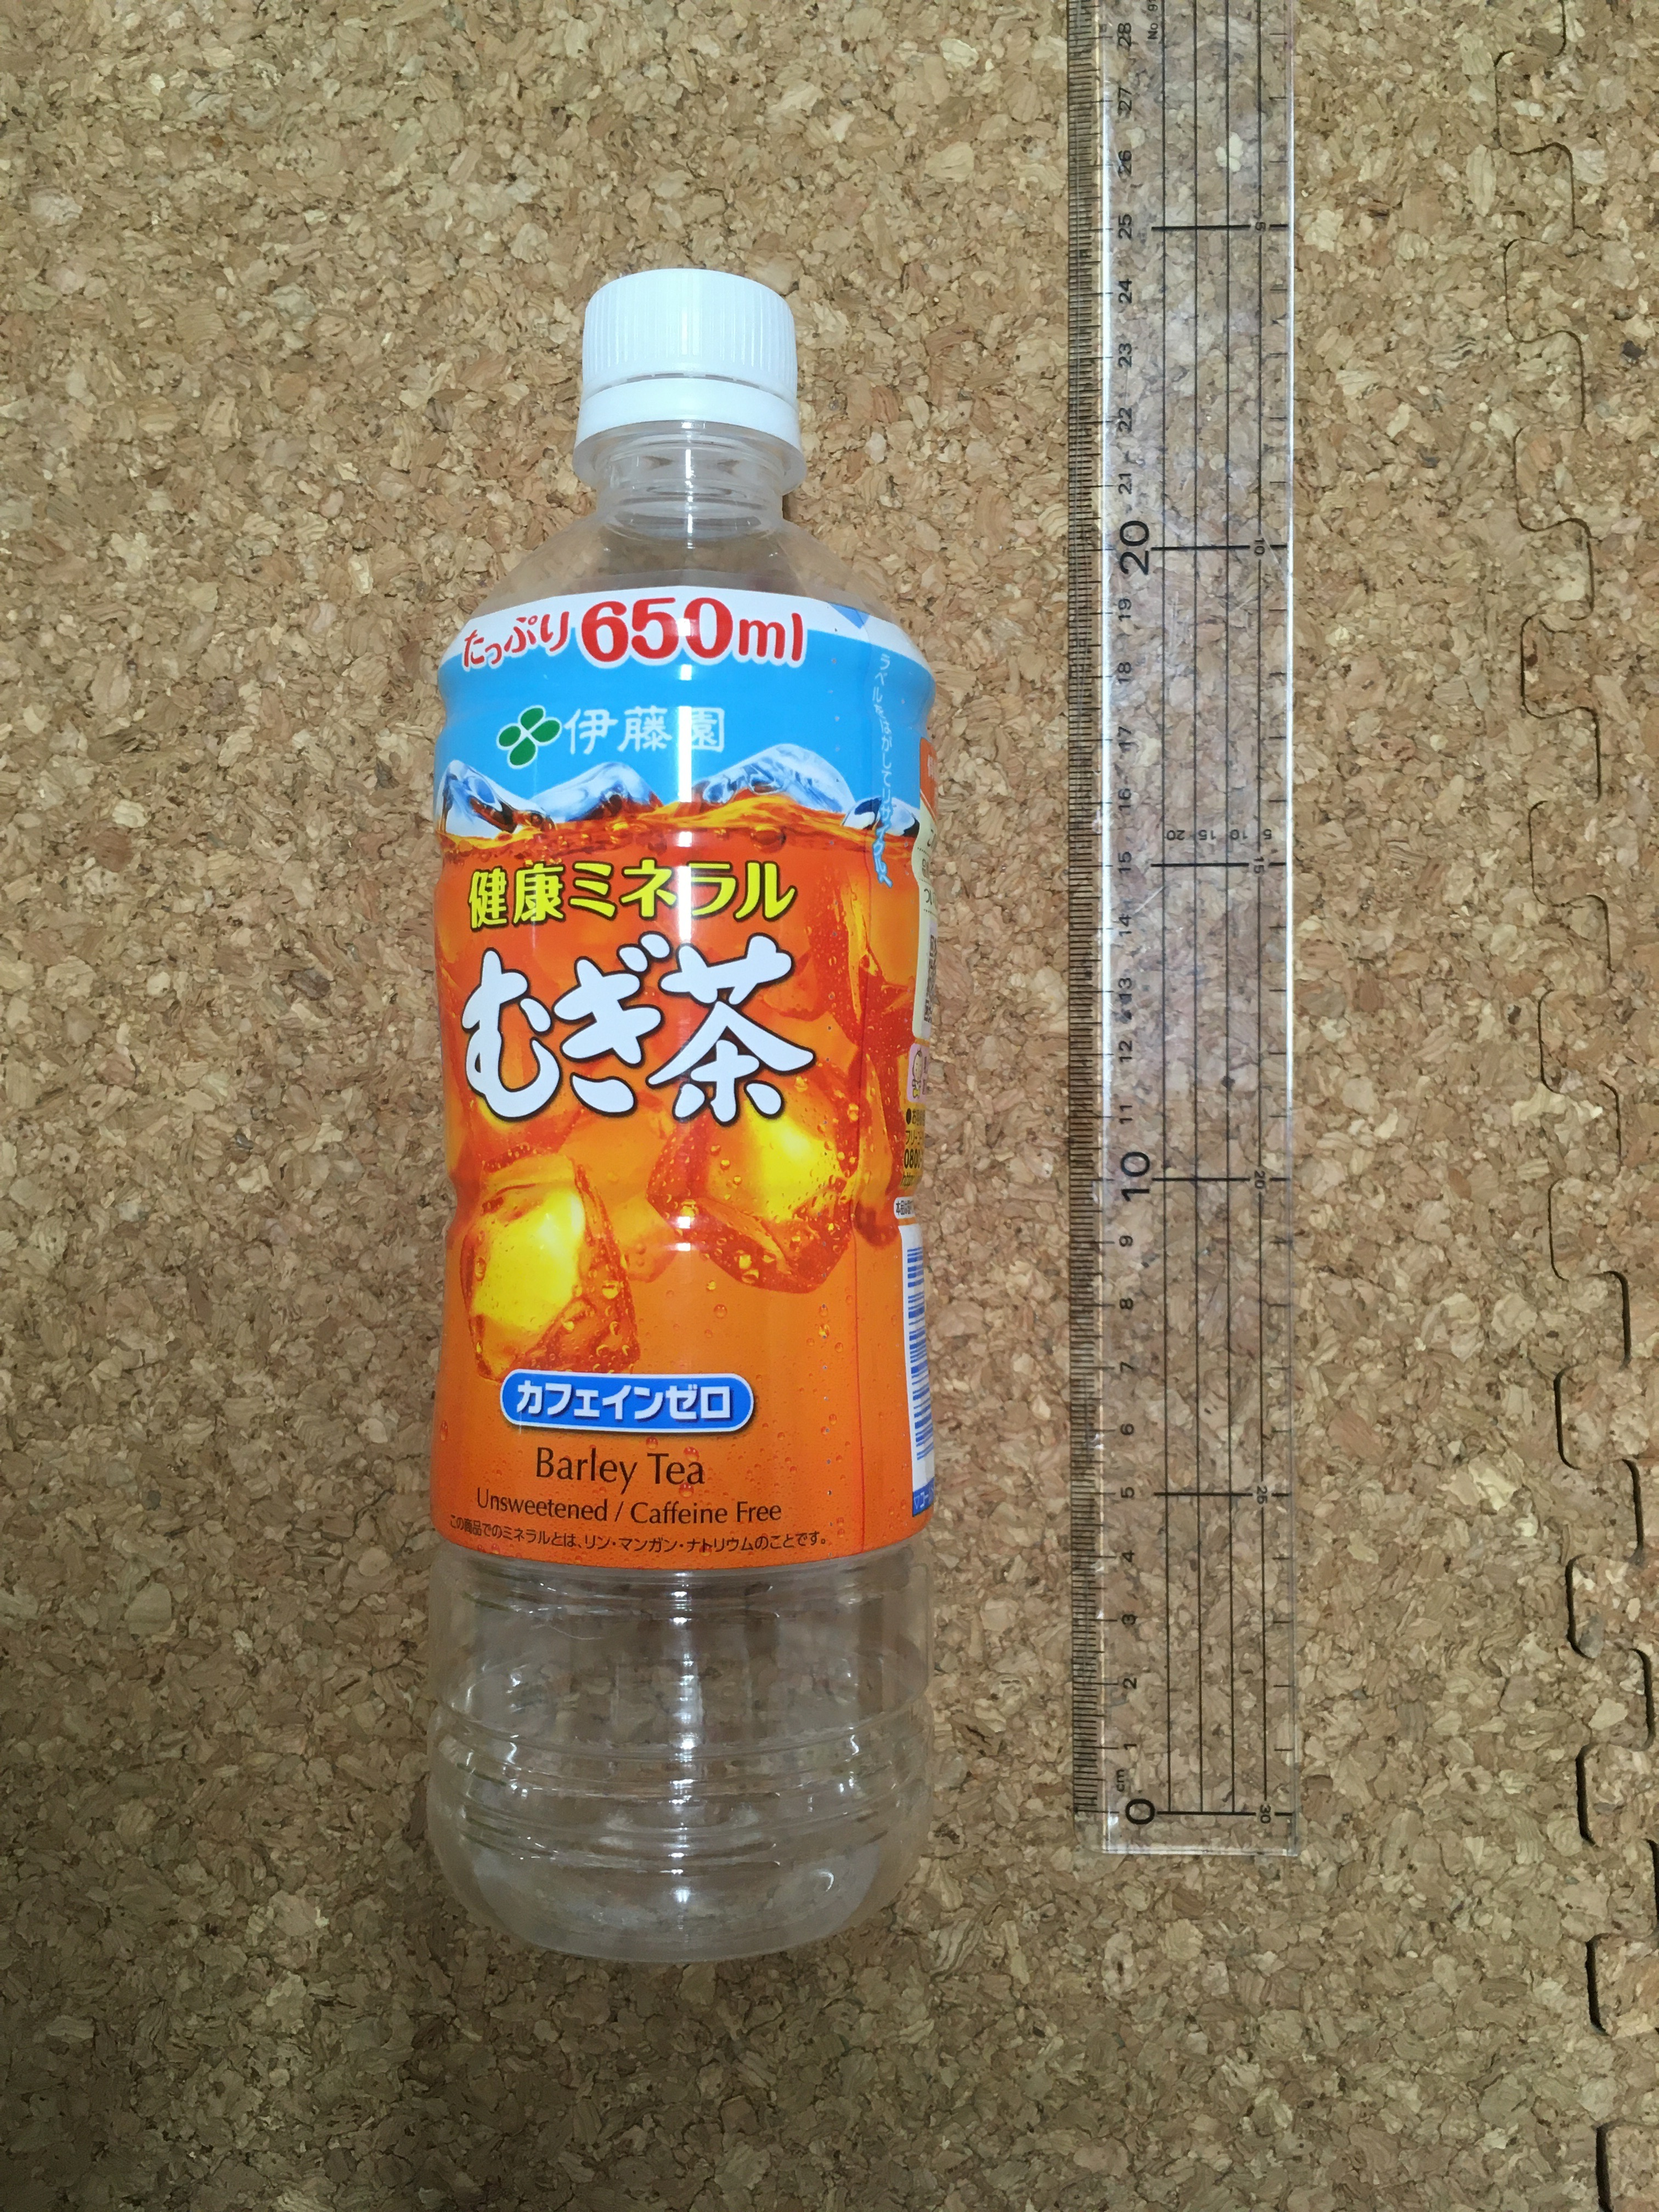
\includegraphics[clip, width=\linewidth]{figure/chapter4/bottle_650ml}
        \subcaption{bottle(350ml)}
    \end{minipage}
    \begin{minipage}{0.19\columnwidth}
        \centering
        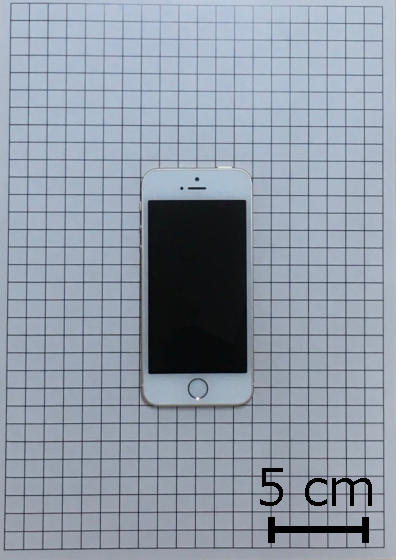
\includegraphics[clip, width=\linewidth]{figure/chapter4/cellphone}
        \subcaption{cell phone}
    \end{minipage}
    \begin{minipage}{0.19\columnwidth}
        \centering
        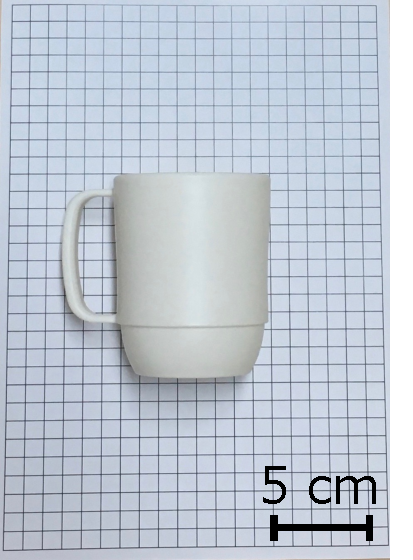
\includegraphics[clip, width=\linewidth]{figure/chapter4/cup2}
        \subcaption{cup}
    \end{minipage}
    \begin{minipage}{0.19\columnwidth}
        \centering
        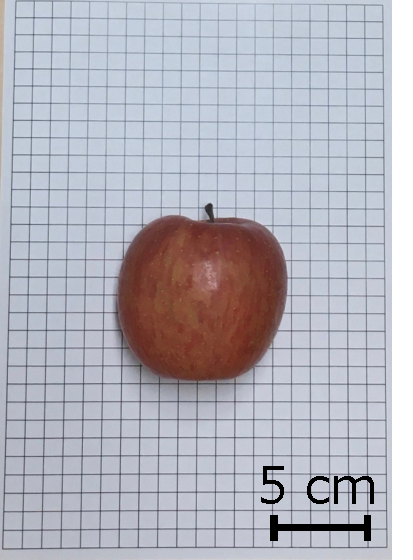
\includegraphics[clip, width=\linewidth]{figure/chapter4/apple}
        \subcaption{apple}
    \end{minipage}

    \caption{Objects.}
    \label{fig:対象物}
    
\end{figure}

\begin{table}[H]
    \centering
    \caption{Details of objects.}
    \begin{tabular}{ccccc}\toprule
        & Size & Weight & \# of Training data & Notes \\ \midrule
        bottle(350 ml) & 16.5 $\times$ $\phi$ 5.9 cm & 26.28 g & \multirow{2}{*}{8880} & Empty \\ 
        bottle(650 ml) & 22.0 $\times$ $\phi$ 6.9 cm & 29.94 g &  & Empty \\ 
        cell phone & 0.78 $\times$ 5.9 $\times$ 12.0 cm & 127.51 g & 5017 & iPhone SE \\ 
        cup & 9.8 $\times$ $\phi$ 7.9 cm & 82.50 g & 9579 & Empty \\ 
        apple & $\phi$ 8 cm & 263.32 g & 1662 & Raw \\ \bottomrule
    \end{tabular}
    \label{tab:対象物}
\end{table}

まず,\ref{sec:mrcnn学習}節で学習を行ったCOCO2014の学習済みモデルを使用してMask R-CNNの識別精度を検証した.また各対象物において,ロボットハンドとの距離すなわち画角によってMask R-CNNの検出精度およびそのクラス分類の精度が異なるかを検証した.

次に,各物体に対して接近成功率および把持成功率を検証した.接近成功率とは,上記実験で決めた物体検出の限界距離まで近づきかつ対象物を正面に捉えて静止したら成功,対象物の正面で止まれなかったら失敗とし,10回試行したときの成功率とした.把持成功率とは5秒間持ち上げ続けたら成功,そうでなければ失敗とし,10回試行したときの成功率とした.
接近および把持のタスクは以下のように定めた.タスク1が接近タスクでタスク2が把持タスク,タスク1+タスク2が接近・把持の一貫タスクである.
\begin{itemize}
    \item タスク1\\
    離れたところに対象物を置き,上記実験で決めた物体検出の限界距離(\ref{sec:識別性能評価}より16 cm)まで接近する.
    \item タスク2\\
    対象物の向かい(物体検出の限界距離16 cm)の場所から把持動作を行う.
    \item タスク1+タスク2\\
    離れたところに対象物を置き,デプスの測定限界距離(17 cm)まで接近し,そこから把持動作を行う.
\end{itemize}


\section{結果}
\subsection{識別性能評価}\label{sec:識別性能評価}
正立させた"bottle"はどの向きにおいても検出できた."cell phone"はエッジ部分だけでは検出できず,画面側と背面のみ検出できた."cup"は取っ手が写っている角度では検出できたが,取っ手が写らない向きでは"bottle"と誤認識することがあった."apple"はどの向きにおいても検出できなかった.

各対象物において,識別精度の対象物依存性を\fig{mrcnn距離}に示す.なお,"apple"は全ての場所・向きにおいて認識できなかったため載せていない.
\begin{figure}[H]
    \centering
    \begin{minipage}{0.45\columnwidth}
        \centering
        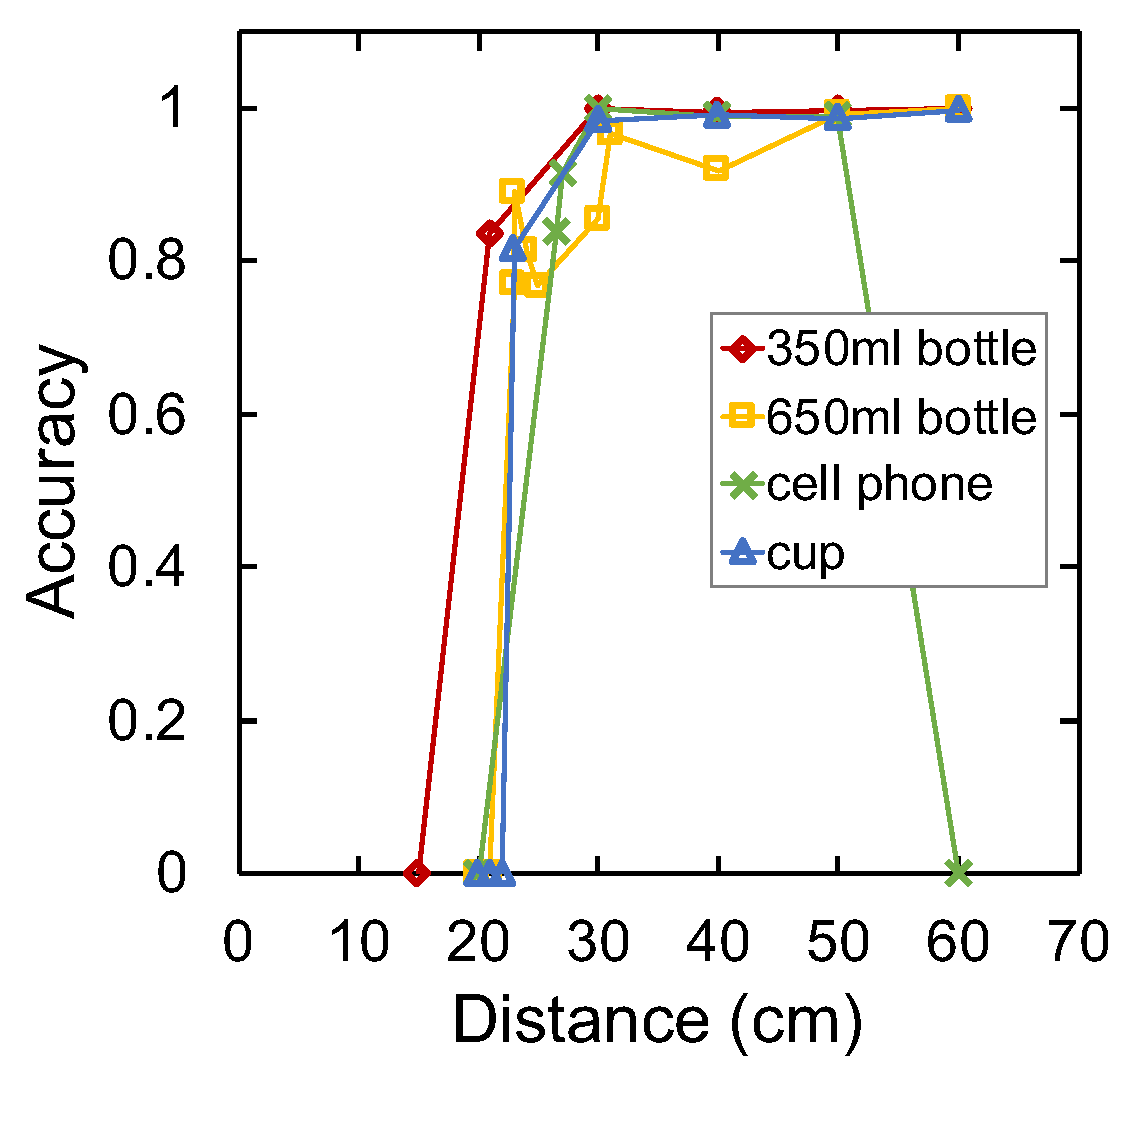
\includegraphics[width=0.95\linewidth]{figure/chapter4/mrcnn_depth}
        \subcaption{Input raw image.}
        \label{fig:mrcnn距離そのまま}
    \end{minipage}
    \begin{minipage}{0.45\columnwidth}
        \centering
        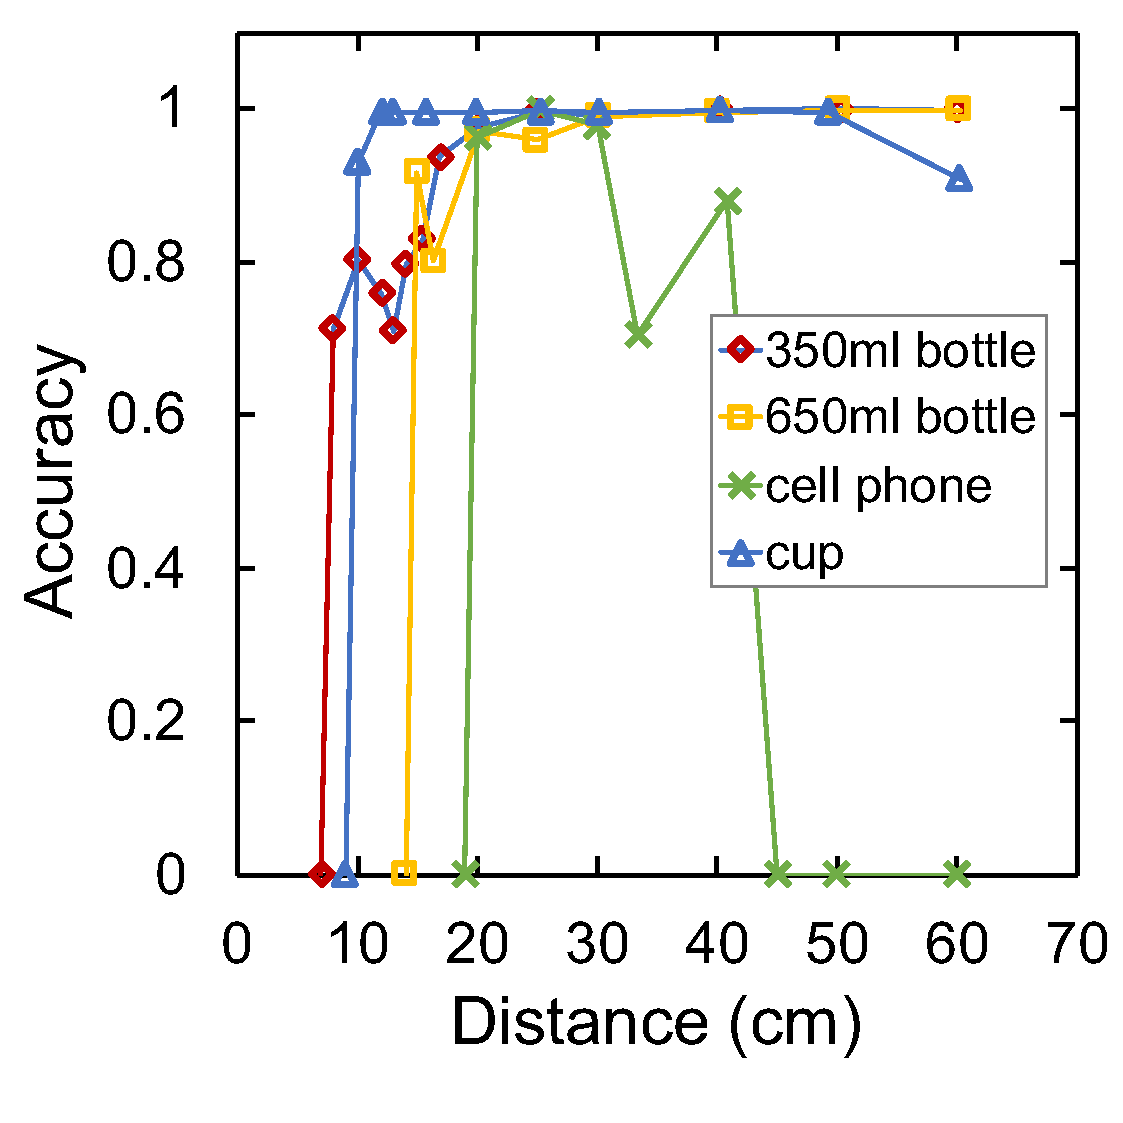
\includegraphics[width=0.95\linewidth]{figure/chapter4/mrcnn_depth_padding}
        \subcaption{Input zero padding image.}
        \label{fig:mrcnn距離パディング}
    \end{minipage}
    \caption{Dependency of distance between camera and object.}
    \label{fig:mrcnn距離}
\end{figure}
カメラ画像をそのままMask R-CNNの入力とした結果が\fig{mrcnn距離そのまま}である.対象物とカメラとの距離が23 cmを境に識別精度が上昇し,30 cm以上では精度がほぼ100\%であることが分かった.しかし,"cell phone"は50 cmよりも遠いと検出できなくなった.

背の高い"bottle(650 ml)"は,距離が近いと画像内に物体全体が収まらず検出精度が下がると予想できるが,背の低い"cup"も同じように精度が下がった.これは学習データに大きく写っている画像が無いことが原因と考えられる.
そこで,入力画像をzero paddingして対象物を小さく写るようにして入力した結果が\fig{mrcnn距離パディング}である.paddingをすることで大幅に距離依存性が改善され,16 cmまで近づいても検出されるようになった.したがって,接近タスクでは16 cmを閾値としてそこまで近くタスクとした.

\subsection{把持タスク評価}
各タスクにおける成功率を\tab{把持成功率}に示す.
\begin{table}[H]
    \centering
    \caption{Success rate on grasping objects tasks.}
    \begin{tabular}{cccc}\toprule
        Objects & Task1 & Task2 & Task1 + Task2 \\ \midrule
        bottle (350 ml) & 60\% & 90\% & 50\% \\
        bottle (650 ml) & 60\% & 80\% & 50\% \\
        cell phone & 60\% & 50\% & 40\% \\ 
        cup & 70\% & 50\% & 30\% \\ \bottomrule
    \end{tabular} 
    \label{tab:把持成功率}
\end{table}
"apple"は認識ができなかったため,全てのタスクにおいて成功率は0であった.

失敗例は,掴み方が悪く掴んでも落とした,掴んで持ち上げたがロボットハンド自体が横転した,持ち上げたがズレ落ちた,などであった.

またホームポジションに戻る動作も実装した.ARマーカーを原点の壁に設置しておき,把持が成功したら旋回してARマーカーを探索し,マーカーを捉えたらそこへ直進した.


\section{考察}
まず,認識性能について述べる.
Mask R-CNNの検出精度における対象物との距離依存性では,対象物の高さに関係なく30 cmから精度が落ち始め,20 cmでは全ての物体で検出できなくなった(\fig{mrcnn距離そのまま}).背の高い"bottle(650 ml)"は,距離が近いと画像内に物体全体が収まらず検出精度が下がると予想できるが,背の低い"cup"も同じように精度が下がった.これは学習データに大きく写っている画像が無いことが原因と考えられる.
そこで,入力画像をzero paddingして対象物を小さく写るようにして入力した結果が\fig{mrcnn距離パディング}である.paddingをすることで大幅に距離依存性が改善され,16 cmまで近づいても検出されるようになった.

次に,把持性能について述べる.
把持成功率より接近成功率が低い原因は,2号機のRGBカメラの位置だと考えられる.2号機に搭載したカメラRealSenseは左端にRGBカメラ,真ん中右寄りにデプスカメラが付いているため,RGB画像は右側を見ることが難しい.そのため,ロボットハンドから距離が離れていれば問題ないが,対象物がロボットハンド近接時において右側に位置すると死角となり,認識不能となり接近できないという事になる.また,"cell phone"と"cup"は把持成功率が低く,"bottle"の把持成功率が高い理由としては,把持対象物の対称性が考えられる.bottleは円筒対称であるため,どの角度からアプローチしても同じ把持が可能だが,"cell phone"や"cup"は"bottle"より対称性が悪いため,ルールベースでは正しい位置で把持できなかった.これは各物体に対して把持位置を学習するなど,より高度なアルゴリズムが必要となる.また,非対称性の複雑な形状をもつ物体の把持が可能なJamming転移型グリッパ\cite{jamminggripper}や多指グリッパ,吸盤グリッパなどへの変更も選択肢である.

"apple"が認識できなかった原因は,学習データ数の偏りにあると考えられる.\tab{対象物}に示したように,"apple"だけ他の対象物よりも訓練データが3分の1以下と少ない.したがって今回使用したモデルは"apple"の認識が弱いモデルだったと考えられる.


\section{まとめ}
物体の識別(インスタンス認識)をし,対象物の把持およびその次の動作を可能とするロボットハンドを実現するため,機構の多自由度化を行い,深層学習を用いた物体検出を用いたロボットハンドを作製した.
物体検出では,データセットの特性を考えて入力画像をpaddingすることで,対象物とカメラの距離が近くても物体を検出できることができるようになった.日常生活によくある物体3種類の物体を認識し,接近・把持を行い,物体を持ち上げて運搬することを可能とし,ペットボトルの把持成功率は9割に達した.

2号機の課題として,計算リソースの都合上,GPUを搭載したデスクトップPCと有線で接続されているため,携帯性が低下した.また,ロボットハンドの重量が軽いために,ロボット本体重量以上の重い物体を持ち上げることができなかった.